\section{Experiments}
\label{sec:experiments}
The following section details the implementation of our approach, as well as the parameter values used. We then outline the image datasets that we evaluate and the baselines methods used to compare performances.

\subsection{Implementation and Computational cost}
Our \KSP ~method is implemented in Python/C++\footnote{We make our implementation, along with the tested datasets and corresponding manual ground truth segmentations available at \label{fn:website}\href{www.gazelabel.com}{www.gazelabel.com}}.
The C++ part (see Alg. \ref{alg:ksp}) uses the C++ Boost Graph library \cite{sick02} which includes the Dijkstra and Bellman-Ford algorithm.
Using a Linux machine equipped with a Quad-core 3.2 GHz Intel CPU, the construction of both the forward and backward graphs take 15 minutes each.
Superpixel segmentation, including the extraction of dense optical flow, requires 10 minutes.
Each iteration in Alg.~\ref{alg:iter_ksp} takes 5 minutes, including the training of the classifier and computing the entrance-exit models.
The number of KSP iterations varies between 1 and 5 depending on the sequence and the provided 2D locations.
A GeForce GTX 1080 Ti GPU and a PyTorch \cite{pytorch} based implementation of our network was used for our IOS features, taking ~1 hour per sequence.

In total, our method therefore takes roughly 2 hours for a sequence of 120 frames.

\subsection{Selection of Parameters}
Table~\ref{tab:parameters} specifies the values of the parameters used in the experiments that follow.
Note that these are fixed once and for all, over all experiments and for all datasets. These values were selected empirically so to perform well over all tested sequences.

\begin{table}[htbp]
\centering
\begin{tabular}{c p{8cm} c }
\toprule
Symbol & Description & Value \\
\toprule
$N_t$   & Approximate number of superpixels per frame & $520$\\
$M$   & Number of trees of bagging classifier& $500$ \\
$\tau_{\rho}$   & Threshold on probabilities of foreground model & $0.5$\\ 
$\tau_{u}$   & Threshold on histogram intersection cost & $0.75$ \\ 
$\tau_{trans}$  & Threshold on appearance-transition probabilities & $0.9$\\
$k$ & Number of clusters for LFDA & $5$\\ 
$D$ & Number of dimensions for LFDA & $7$\\ 
$R$   &Normalized radius of entrance/transition neighborhood & $0.05$ \\ 
$\sigma_{g}$  & Normalized standard-deviation for prior in feature extraction & $0.3$ \\
\bottomrule
\end{tabular}
\caption{Summary of the parameters used in \KSP.}
\label{tab:parameters}
\end{table}

\subsection{Datasets}
\label{sec:data}
We evaluate our method on a mixture of datasets consisting of video sequences and volumetric images. Note that the datasets include a variety of different image modalities with a wide range of applications. The singularities of each sequence are given so as to emphasize the flexibility of our method. Note that for each sequence and for all datasets, a single object of interest is present on any give image:

\begin{itemize}
\item[-]{\bf{Brain:}} $4$ randomly selected volumetric sequences from the publicly available BRATS challenge dataset \cite{menze15}. Each volume contains a 3D  T2-weighted MRI scans of a brains containing a tumor, which we choose as the object of interest. The tested volumes contain ${73,69,75,74}$ slices each of size ($240 \times 240$). Tumors have in general a ball-like shape, \ie their radius increases and decreases as slices unfold.

\item[-]{\bf{Tweezer:}} We extract $4$ sequences from the training set of the publicly dataset MICCAI Endoscopic Vision challenge: Robotic Instruments segmentation \cite{endochal}. Each extracted sequence contains $121$ frames and are acquired at $25$ fps. The object to segment in each sequence is a surgical instrument, and where each frame is of size ($640 \times 480$). The tool is piecewise-rigid and is subject to translations and rotations in an otherwise stable environment.
  
\item[-]{\bf{Slitlamp:}} $4$ slit-lamp video recordings of human retinas, where the optic disk must be segmented. The sequences contain ${129,121,75,130}$ frames of size ($680 \times 512$), all acquired at 25 fps. The object has a relatively constant shape and texture, but  undergoes abrupt translations occasionally. Due to this imaging technique, the background also changes lighting abruptly, with non-global bright beams of yellow and blue light appearing.

\item[-]{\bf{Cochlea:}} $4$ volumes of 3D CT scans of the inner ear, where the cochlea must be annotated. The challenge with this dataset lies in the fact that the object of interest branches out in several parts and merges back. Volumes contain ${99,96,116,104}$ slices of size ($300 \times 290$).
\end{itemize}

For the {\bf Slitlamp} and {\bf{Cochlea}} datasets, we manually segmented the object ground truth on each frame in each image sequence. Manual pixel-wise annotations are publicly available for the {\bf Brain} and {\bf Tweezer} datasets. The complete set of used image sequences and manual ground truths are publicly available \footref{fn:website}.

\subsection{Generating 2D coordinate locations}
Unless otherwise specified, 2D coordinate locations, $g_t$ for each sequence were collected using an off-the-shelf gaze tracker (Eye Tribe Tracker, Copenhagen, Denmark) as in~\cite{lejeune17}. To do this,  the tracker was placed beneath a $12.3"$ tablet roughly $50cm$ away from a user's face. For each recording session, an initial calibration procedure was performed using the inbuilt software of the tracker and validated before all gaze information recordings took place, allowing less than 1$^{\circ}$ tracking accuracy at 30fps.

Gaze recordings were then collected by a domain expert who had been instructed to observe the object of interest throughout the sequence. During the displaying of the video, gaze locations were recorded using a dedicated software\footref{fn:website}. Videos were displayed at $10$ fps and 2D locations were then taken to be the average ($x,y$) coordinates given by the tracker over the corresponding time interval. As such, excluding the initial calibration phase, annotating a 100 frame sequence with a single 2D location per frame took roughly 10 seconds. 

\subsection{Baselines}
To compare our approach to existing methods in the literature, we evaluate the following closest methods:

\begin{itemize}
\item[-]{\PSVM :} Patch-based SVM
is a transductive learning approach \cite{vilarino07} explicitly developed to use gaze information to produce \blue{segmentations} when viewing endoscopy video sequences.

\item[-]{\GS :} This approach used gaze trackers to annotate CT volumes using a saliency map-construction and a Random-Walker to segment the object of interest \cite{khosravan16}.

\item[-]{\EEL :} An expected exponential loss was proposed to learn robust classifiers in a PU learning setting \cite{lejeune17}. As in this paper, the method is presented over a variety of image datasets and used a gaze tracker to specify 2D coordinates.

\item[-]{\DL :} Point location supervision was used to train a CNN while using a strong object prior to provide additional information to the network \cite{bearman16}. The method was demonstrated to perform well on natural images.
\end{itemize}

To compare these methods, we implemented both \PSVM ~and \GS ~following their description, while we used provided code for \EEL ~and \DL . \PSVM, \GS, \EEL ~and \DL ~require approximately $8, 1, 3, 4.5$ hours respectively to process sequences. This computation time is roughly equivalent to our proposed method.

\section{Results}
\label{sec:results}
To validate our approach across a wide range of settings, we report the following 5 experiments: 
(i) The performance of the proposed method is compared to the baseline methods for all sequences in terms of segmentation accuracy; (ii) we compare the performance of a supervised prediction method when trained with ground truth generated by hand or with our approach; (iii) we assess the robustness of our method with respect to the selection of the 2D locations; (iv) we evaluate our IOS feature extraction strategy and compare it to different alternatives; (v) we assess the robustness of our method with respect to outliers and missing 2D locations.

\subsection{Experiment 1: Accuracy of produced segmentation}
\label{sec:accuracy}
We first compare the accuracy of pixel-wise segmentations produced by our method and the baselines.
We illustrate in Fig.~\ref{fig:ROC-PR} the ROC and Precision-Recall curves for each method and for each dataset. In each case, we show the performance on each sequence (in light color) and averaged over each dataset (in bold). To measure segmentation accuracy, we also compute the F1-score for each method on each sequence and report these values in Table.~\ref{tab:stats}.

In addition, we distinguish our method in two: \KSP ~and \KSPOPT. In the former, we take the output of the method from the optimization directly. In the latter, we use the probabilities provided by our foreground model after training on the solution of \KSP. We then select the best threshold to maximum performance. As such, \KSPOPT ~can be viewed as the optimal segmentation one could hope for if we had a validation set, while \KSP ~uses no additional information to infer any threshold.

We report substantial improvement over all sequences in both categories. On the {\bf Tweezer} sequence, we improve the best baseline by
$196\%$ (\KSP ~vs.~\PSVM ~) and $12\%$ (\KSPOPT ~vs.~\DL). On the {\bf Brain} sequences, we improve by $40\%$ (\KSP ~vs.~\PSVM) and $36\%$ (\KSPOPT ~vs.~\DL).
On the {\bf Slitlamp} sequence, we report an improvement of $108\%$ (\KSP ~vs.~{\bf P-SVM}), and $32\%$ (\KSPOPT ~vs.~{\bf DL-prior}).
Similarly, for {\bf Cochlea}, we improve over the best baseline by $370\%$ (\KSP ~ vs.~\PSVM), and $113\%$ (\KSPOPT ~vs.~\DL).

As illustrated in Fig.~\ref{fig:all}, the results of our methods show improved segmentations compared to tested baselines from a qualitative point of view. To further depict the tracking that our approach produces, Fig.~\ref{fig:brain_paths} shows how the tracklet association of different superpixels across frames in a {\bf Brain} sequence for both the forward and backward passes of the optimization. Here the tumor is initially small (\ie frame 1), then grows (\ie frames 16, 31 and 46) to ultimately shrink again (\ie frame 61). We can see that certain superpixels are tracked over multiple frames even though the number of regions to segment varies across the frames.

\blue{
  Note that the performance of our approach is bounded by the quality of the superpixels used. In particular, some superpixels may contain both foreground and background pixels which reduces the best case performance of our approach. To quantify the impact of the superpixels on the produced segmentations, we were interested in looking at the F1 score if our approach  produced a ``perfect" labeling. To do this, we computed the F1 score between the manual ground truth and the set of positive superpixels when positive superpixels are defined by having more than a given proportion of positive pixels (\ie proportions of $0.25$, $0.5$, $0.75$ and $1$). That is, a proportion of $1$ is when all pixels in a superpixel are in fact positive pixels. Fig.~\ref{fig:sp_limits} illustrates the relation between these proportions and the average best case F1 score for each datasets. From this, we note that even if our method correctly labeled all superpixels, the F1 score would not be $1$. Also, if a strict threshold were to be used to denote positive superpixels (\ie $1$ or no negative pixels in a superpixel), our approach would provide near perfect performances.
}

\begin{table}
  \centering
  \begin{tabularx}{\textwidth}{c @{\extracolsep{\fill}} c cccc cccc}
  %\begin{tabularx}{\textwidth}{cccccc|ccc}
      \toprule
      \multirow{2}{*}{Type} & \multirow{2}{*}{Method} & \multicolumn{4}{c}{F1} &
      & F1 & PR & RC \\
       & & 1 & 2 & 3 & 4 & & mean $\pm$ std& mean $\pm$ std& mean $\pm$ std\\ 
      \fatline
      \dataall{chapters/ksp/tables/Tweezer_self.csv}{Tweezer}
      \dataall{chapters/ksp/tables/Brain_self.csv}{Brain}
      \dataall{chapters/ksp/tables/Slitlamp_self.csv}{Slitlamp}
      \dataall{chapters/ksp/tables/Cochlea_self.csv}{Cochlea}
  \end{tabularx}
\caption{Comparison of quantitative results on all datasets. We report the F1 score for each method on each tested sequence using 4 different 2D gaze sets. In addition, for each sequence type, we give the mean and standard deviation F1, precision (PR) and recall (RC) scores.}
\label{tab:stats}
\end{table}

\begin{figure}[t!]
    \centering
    \begin{subfigure}[b]{0.5\textwidth}
        \centering
        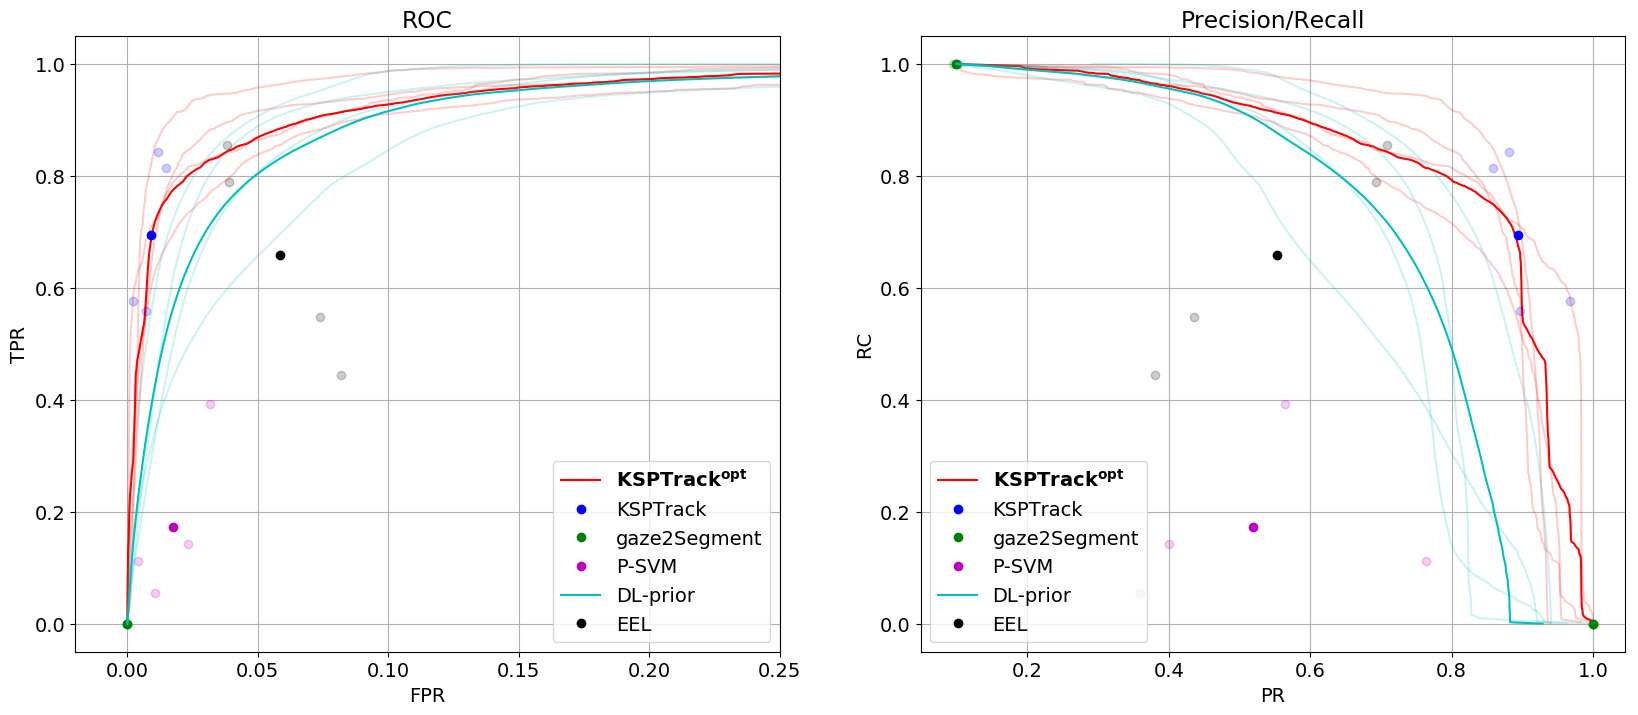
\includegraphics[height=3.5cm]{fig6a}
        \caption{Tweezer}
    \end{subfigure}%
    ~ 
    \begin{subfigure}[b]{0.5\textwidth}
        \centering
        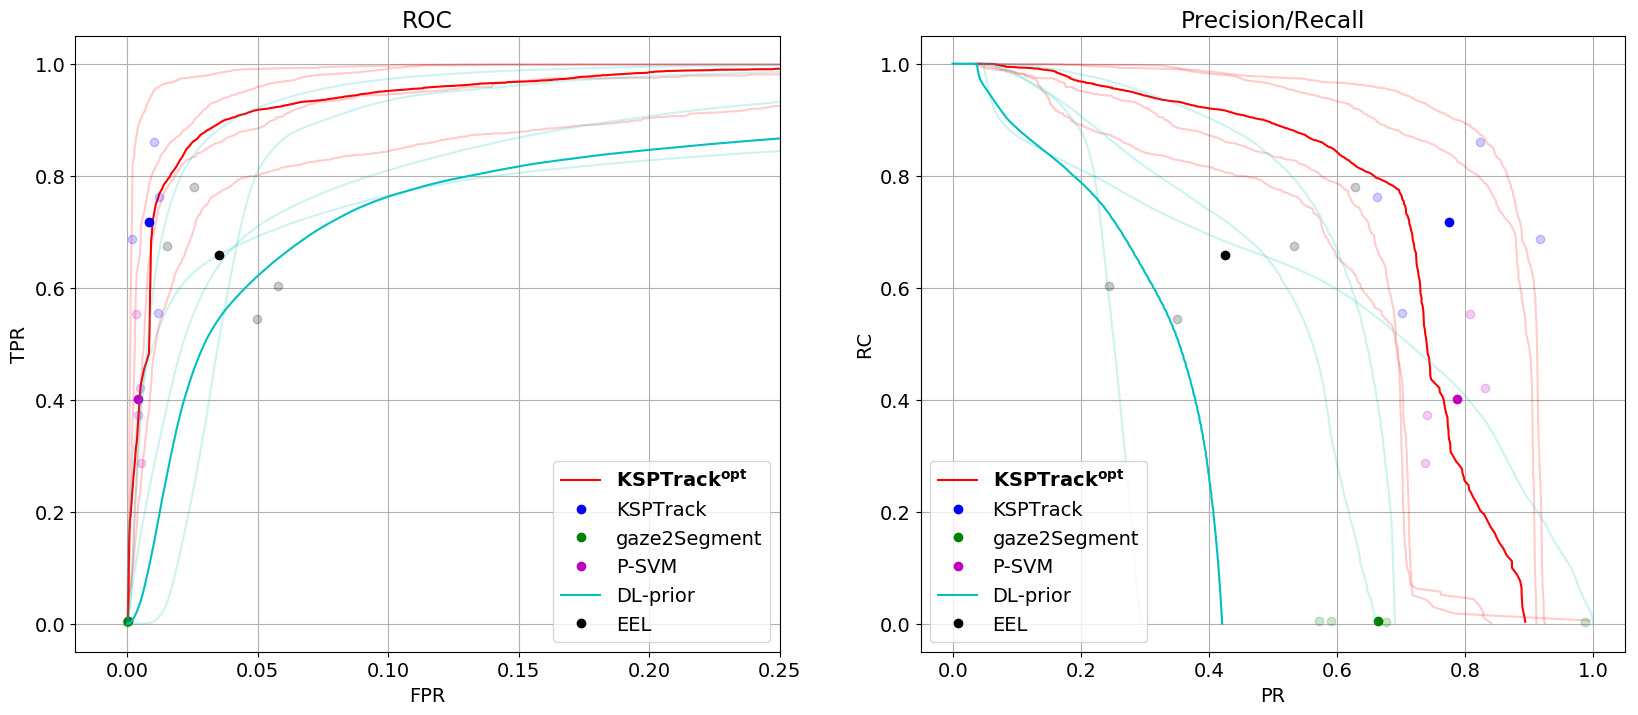
\includegraphics[height=3.5cm]{fig6b}
        \caption{Brain}
    \end{subfigure}
    \begin{subfigure}[b]{0.5\textwidth}
        \centering
        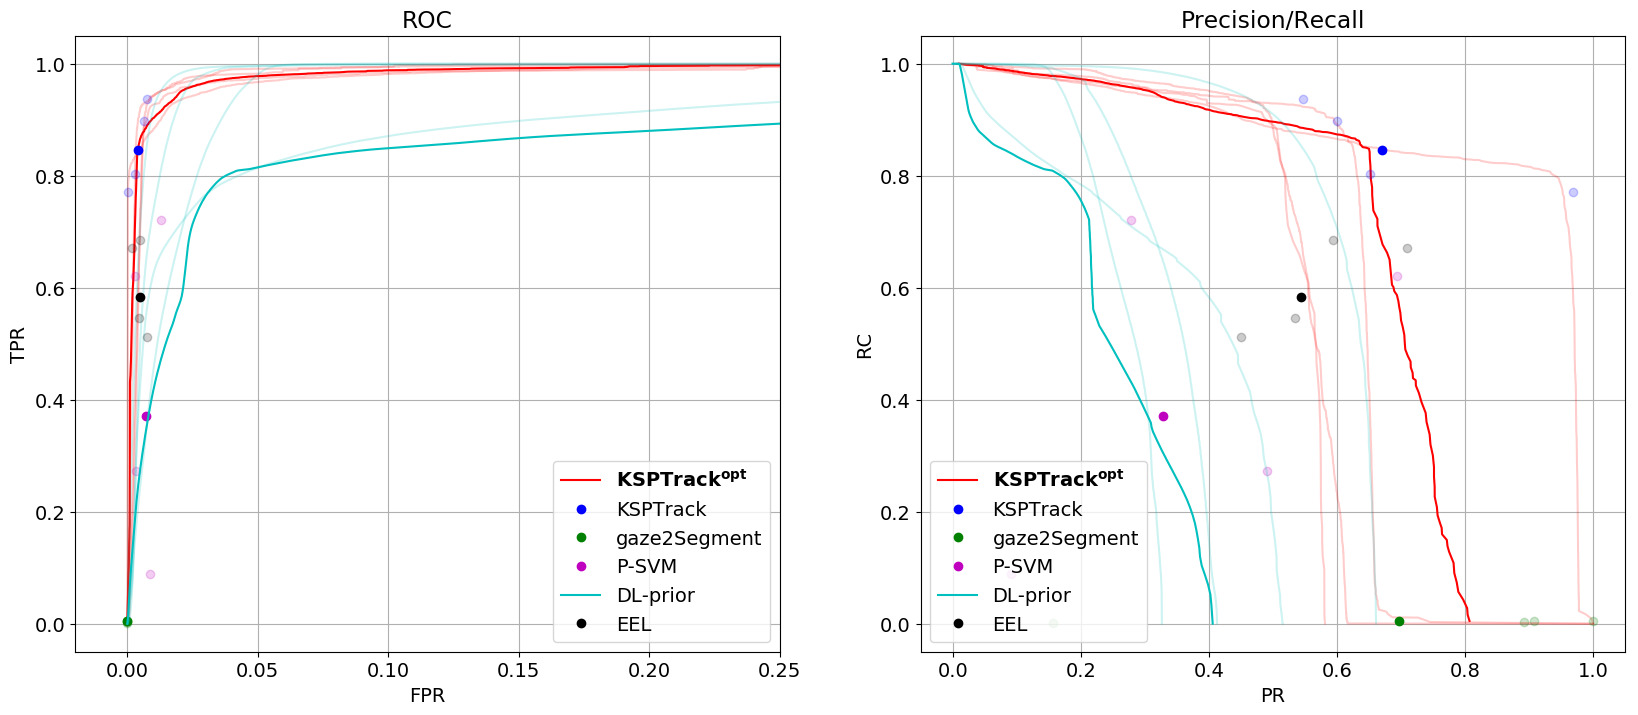
\includegraphics[height=3.5cm]{fig6c}
        \caption{Slitlamp}
    \end{subfigure}%
    ~ 
    \begin{subfigure}[b]{0.5\textwidth}
        \centering
        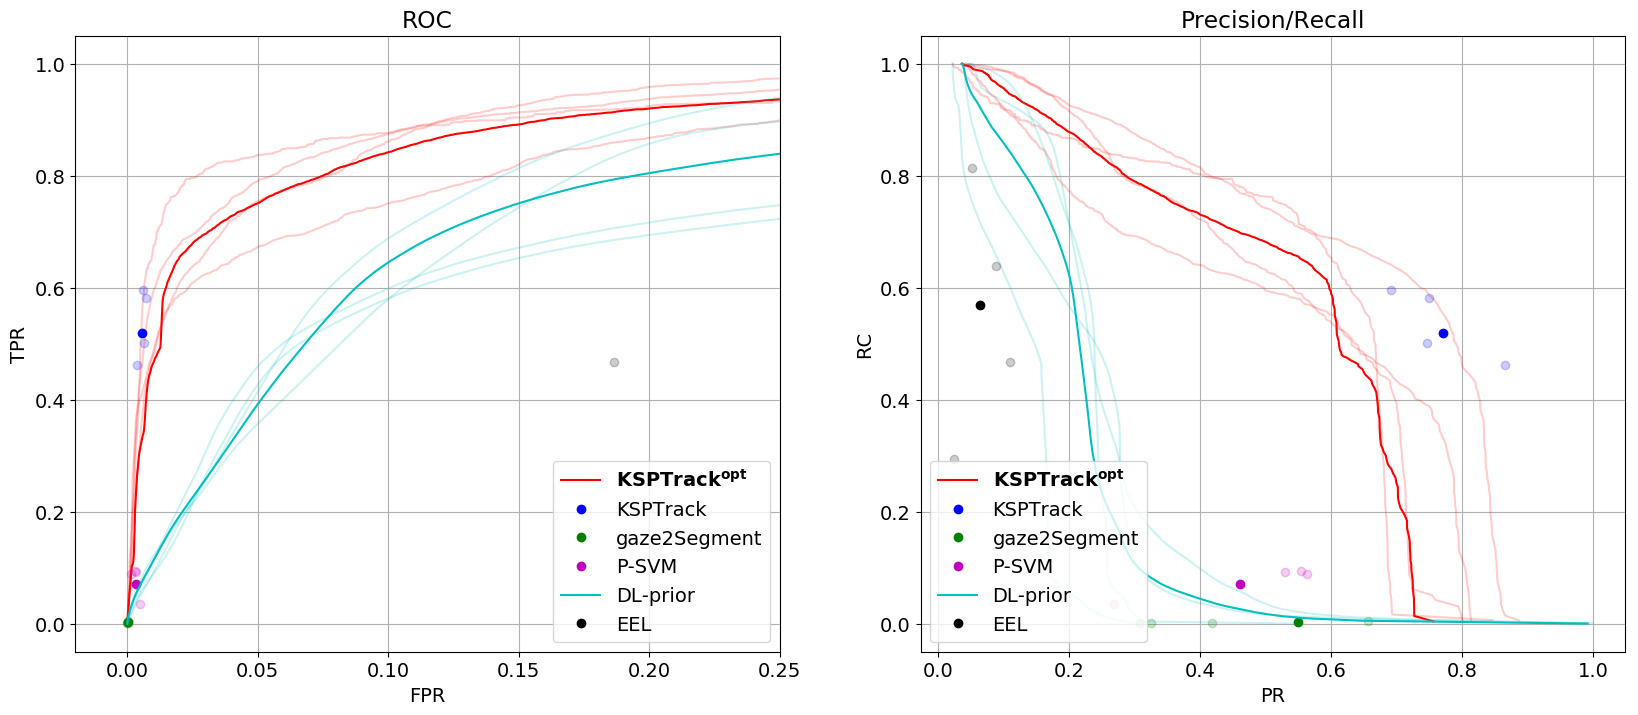
\includegraphics[height=3.5cm]{fig6d}
        \caption{Cochlea}
    \end{subfigure}
    \caption{ROC and Precision-Recall curves for all types of sequence. In each case, we show the performance on each sequence (in light color) and averaged over each dataset (in bold)}
    \label{fig:ROC-PR}
\end{figure}


\begin{figure}
\centering
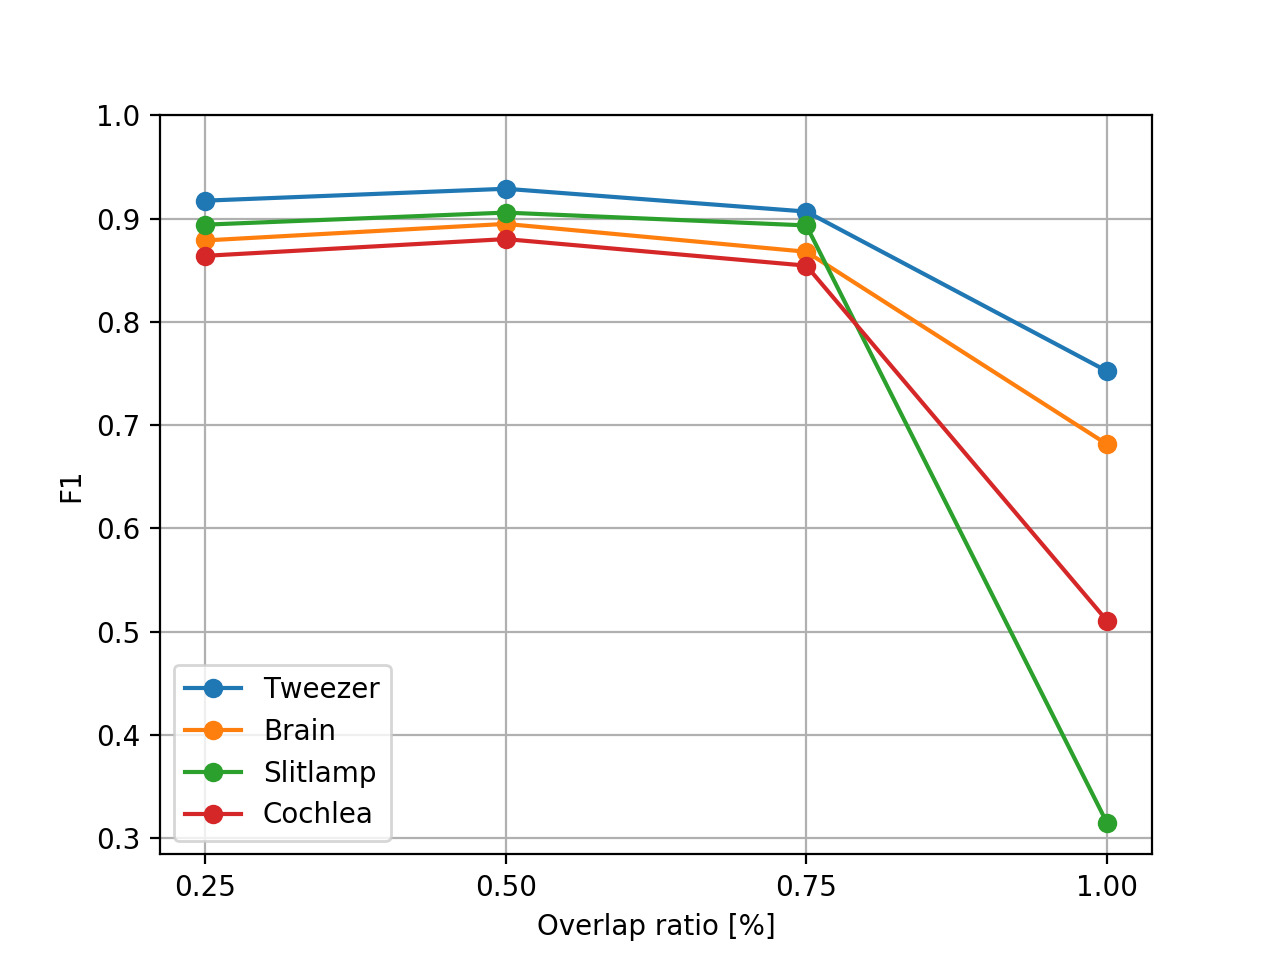
\includegraphics[width=0.5\textwidth]{fig7}
\caption{\blue{Accuracy of superpixel segmentation (F1 score) for each dataset type when using different proportions of positive pixels within a superpixel to define a positive superpixel. F1 scores are averaged over 4 sequences.}}
\label{fig:sp_limits}
\end{figure}

\begin{figure}
\centering
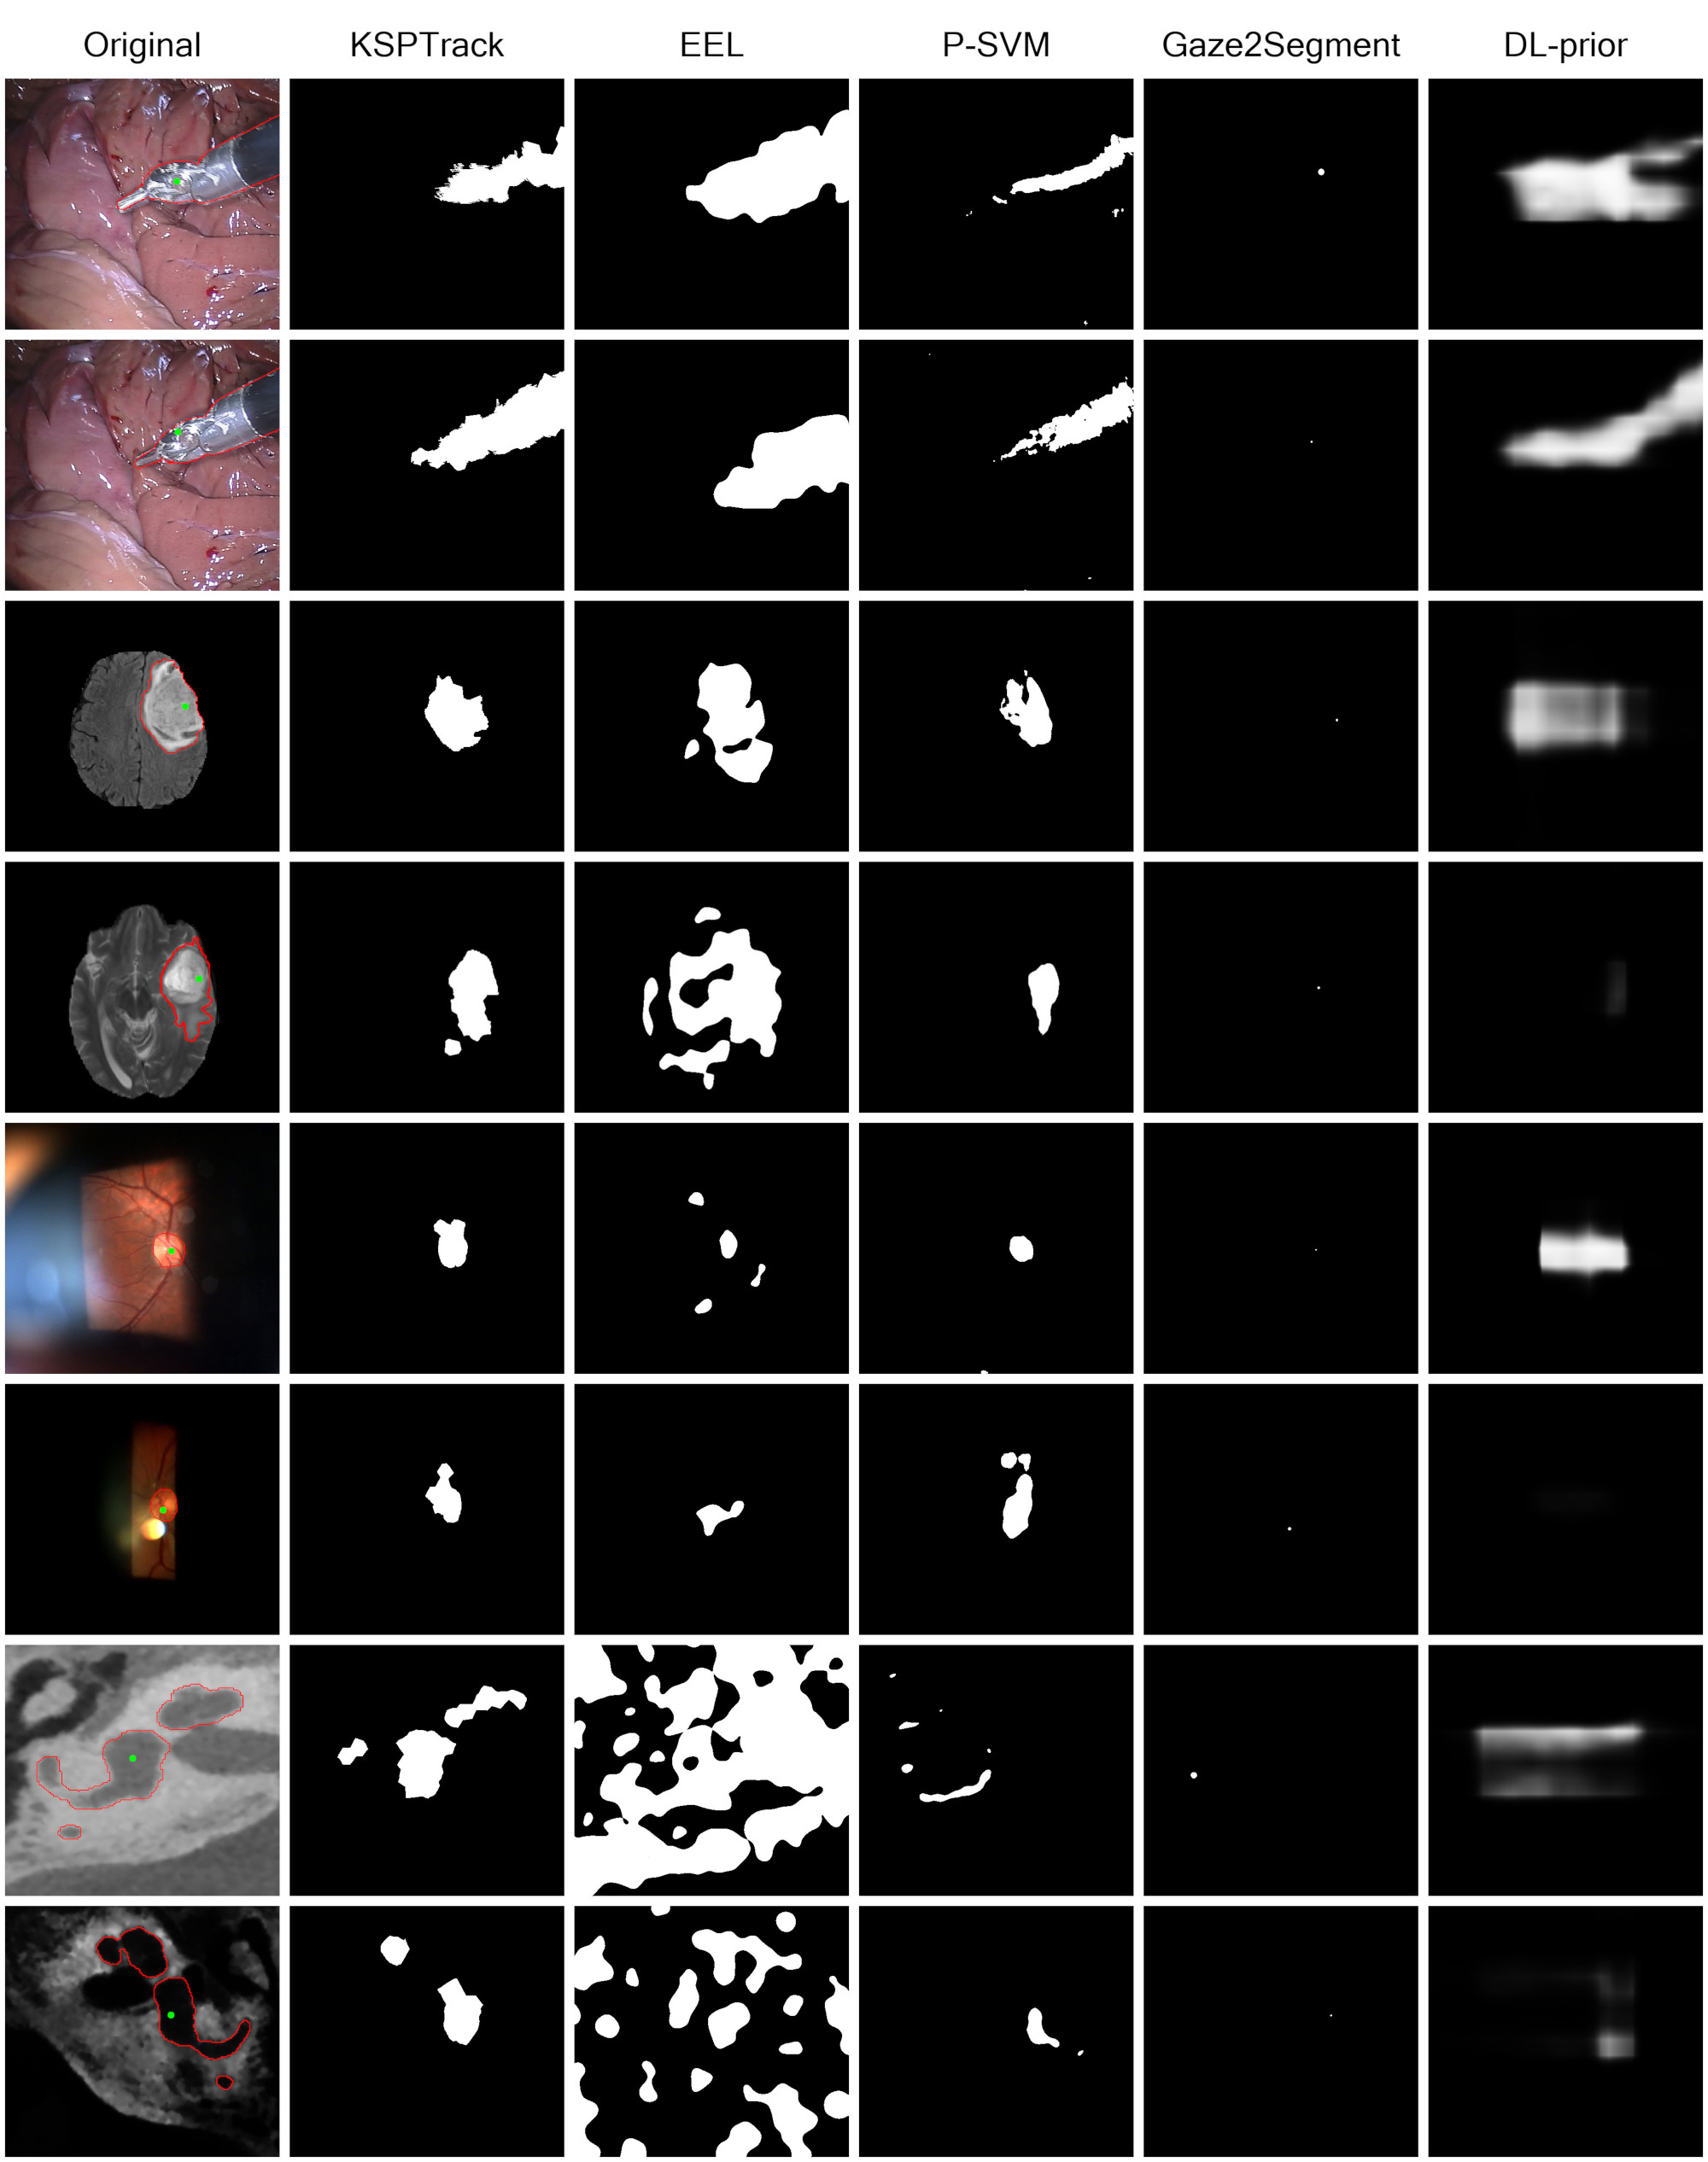
\includegraphics[width=0.99\textwidth]{fig8}
\caption{Qualitative results of compared methods on the tested datasets. (First column) Original image. Ground truth contour of structure of interest is depicted in red and the 2D location is shown in green. (Second row onward) Binary segmentation of methods: \KSPnb ~(Proposed), \EELnb, \PSVMnb, \GSnb, and \DLnb.}
\label{fig:all}
\end{figure}

\begin{figure}[t]
\centering
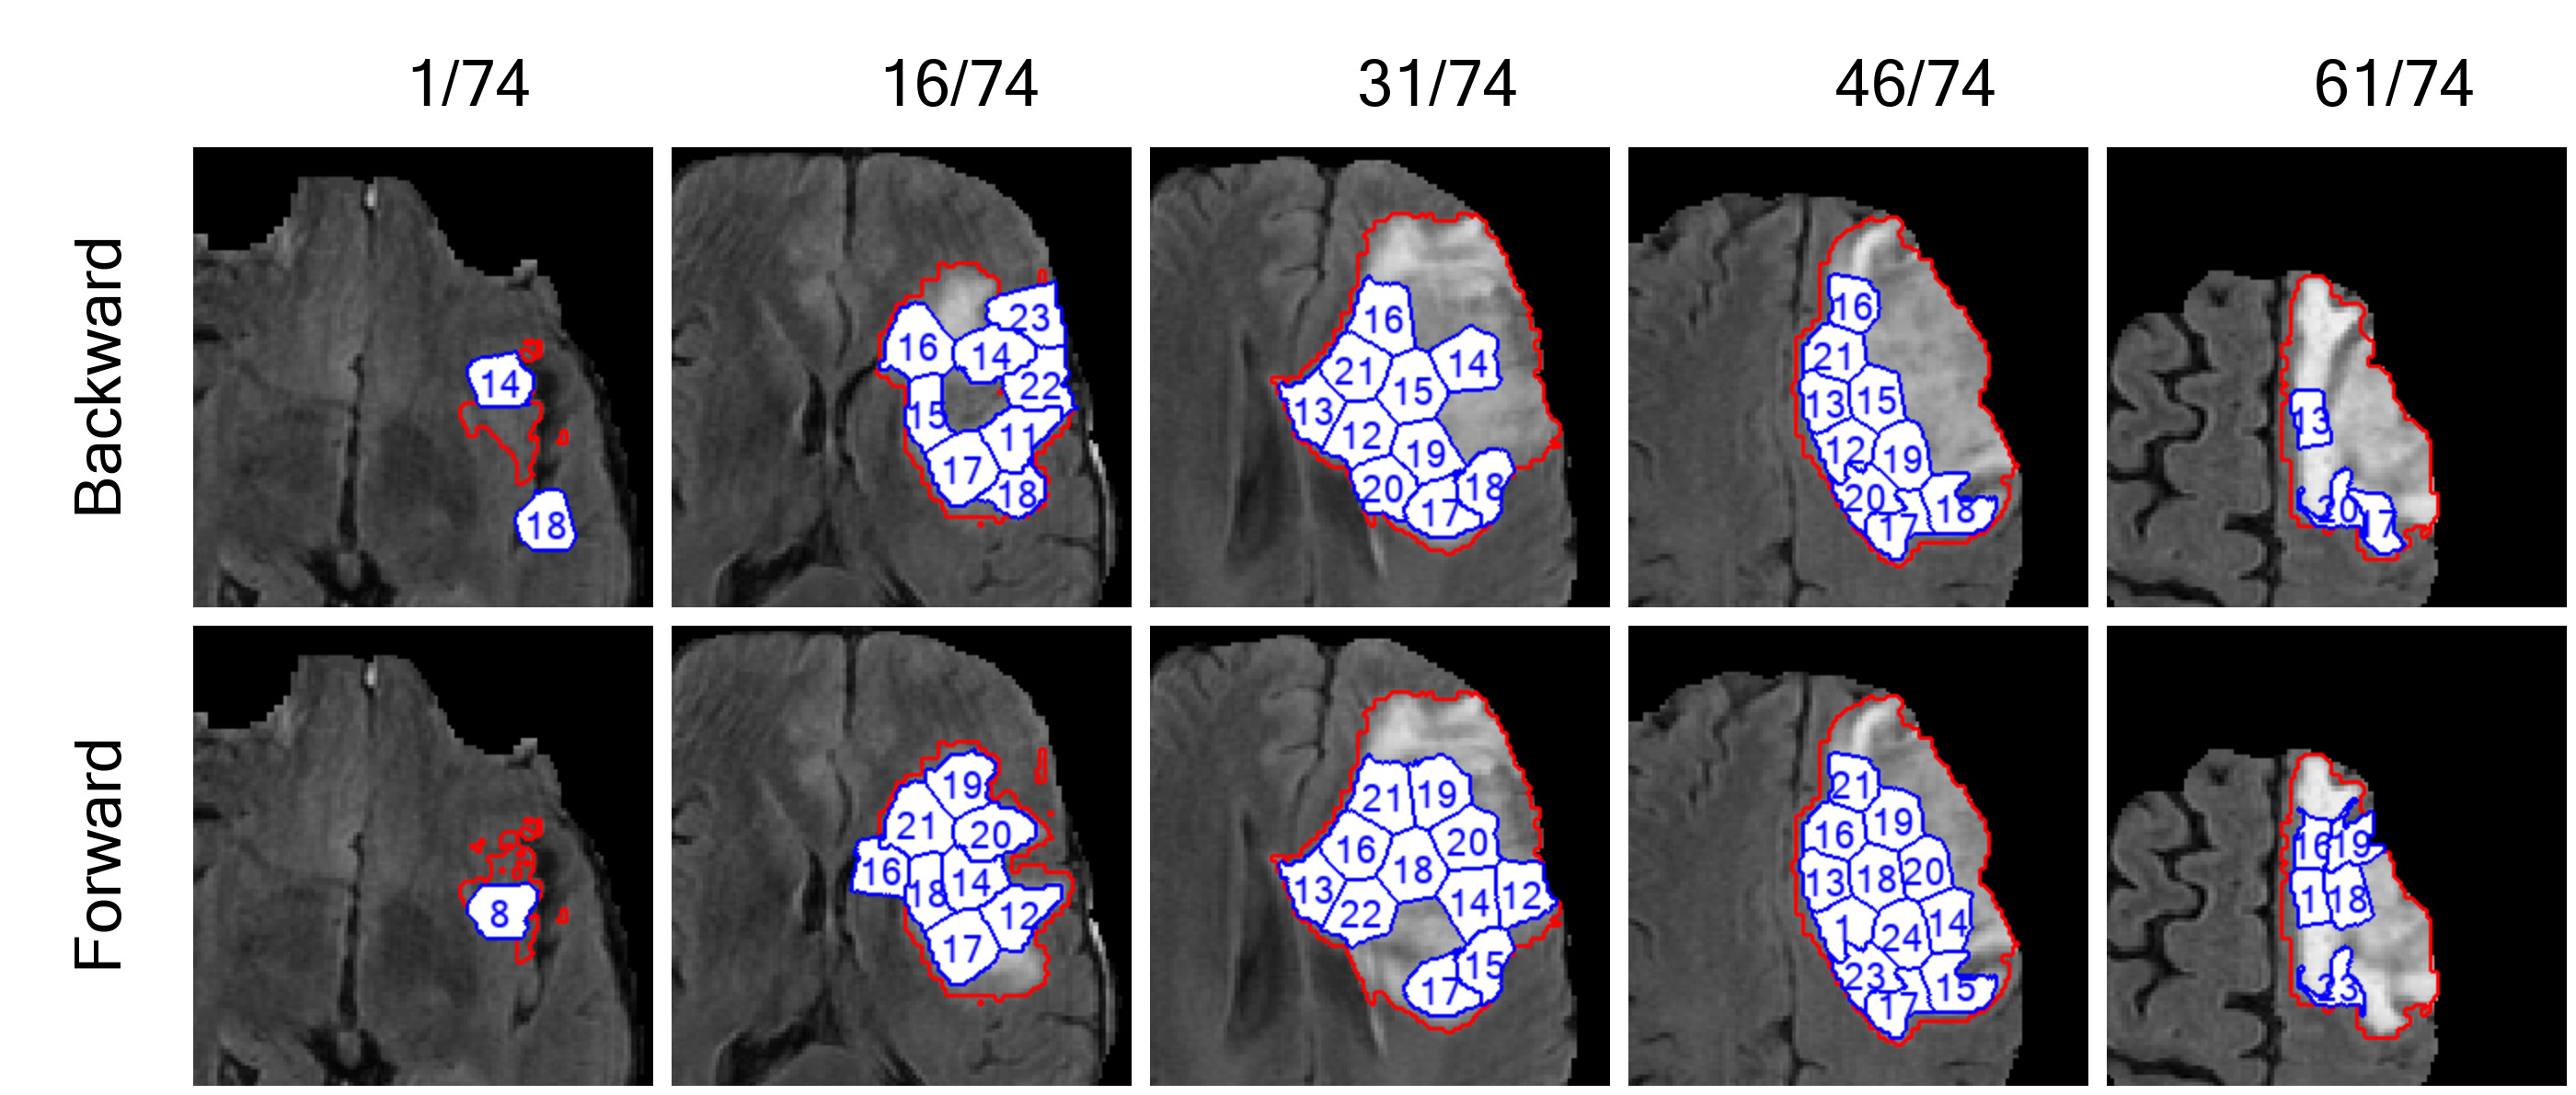
\includegraphics[width=0.99\textwidth]{fig9}
\caption{
Example paths in the forward and backward tracking directions on a Brain sequence. The ground truth is highlighted in red. Segmented superpixels are highlighted in blue. Numbers within superpixel regions denote indices of paths.
}
\label{fig:brain_paths}
\end{figure}

\subsection{Experiment 2: Segmentation performance when using generated \blue{segmentations}}
We now investigate the setting where one wishes to train a segmentation classifier to predict unseen sequences using either manually generated ground truths or \KSP ~produced \blue{segmentations}. That is, we wish to assess the bias of our method may induce by comparing the performance of a classifier that is trained with one type of \blue{segmentation}.

In our experiments, for each dataset, we use 3 out of the 4 sequences to train a standard U-Net using hand-annotated or \KSP ~produced \blue{pixel wise segmentation}. We use the binary cross-entropy as a loss function and perform a leave-one-out prediction (\ie train on $3$ sequences and predict on the last sequence). We keep as validation set $5\%$ of the frames belonging to the train sequence. Each model is trained for $40$ epochs at $500$ iterations per epoch. The model with the lowest validation loss is used in the prediction phase. We compute for each type and each fold the maximum F1-score obtained by both types of segmentations.

Table~\ref{tab:learning} shows the mean scores over the 4 folds when using the hand and \KSP ~\blue{segmentations}, while Fig.~\ref{fig:learning} illustrates example predictions. In particular, we report a gap of $-10\%$ in prediction on the {\bf Tweezer} dataset. The {\bf Brain} sequence shows a gap of $-5\%$. For the {\bf Slitlamp} sequence, a gap of $-16\%$ is obtained. The {\bf Cochlea} sequence shows a gap of $-10\%$.

In general, the fact that our approach provides segmentations that are qualitatively inferior to their hand-based counterpart affects the performance of the classifier in the prediction setup. However, this performance decrease is not overwhelming and depends significantly on the variability of the sequences. In particular, the {\bf Slitlamp} datasets contains a wide range of sequences that appear different from one another. As such, it is not surprising that this dataset suffers the least when compared to the others. 
\begin{table}[h]
\centering
\csvreader[no head,tabular=ccc,
table head=\\\toprule Types & \KSPnb & Manual\\\fatline,
table foot=\hline,
filter expr={
      test{\ifnumgreater{\thecsvinputline}{1}}
    }]
{chapters/ksp/tables/learning_all.csv}
  {1=\type,2=\sksp,3=\smouse}
  {\type & \sksp & \smouse }
\caption{Prediction using manual or produced training annotations. For each type, the mean of the maximum F1 scores for the proposed method (KSP) and the mouse-labeled case are shown.}\label{tab:learning}
\end{table}
\begin{figure}[h]
\centering
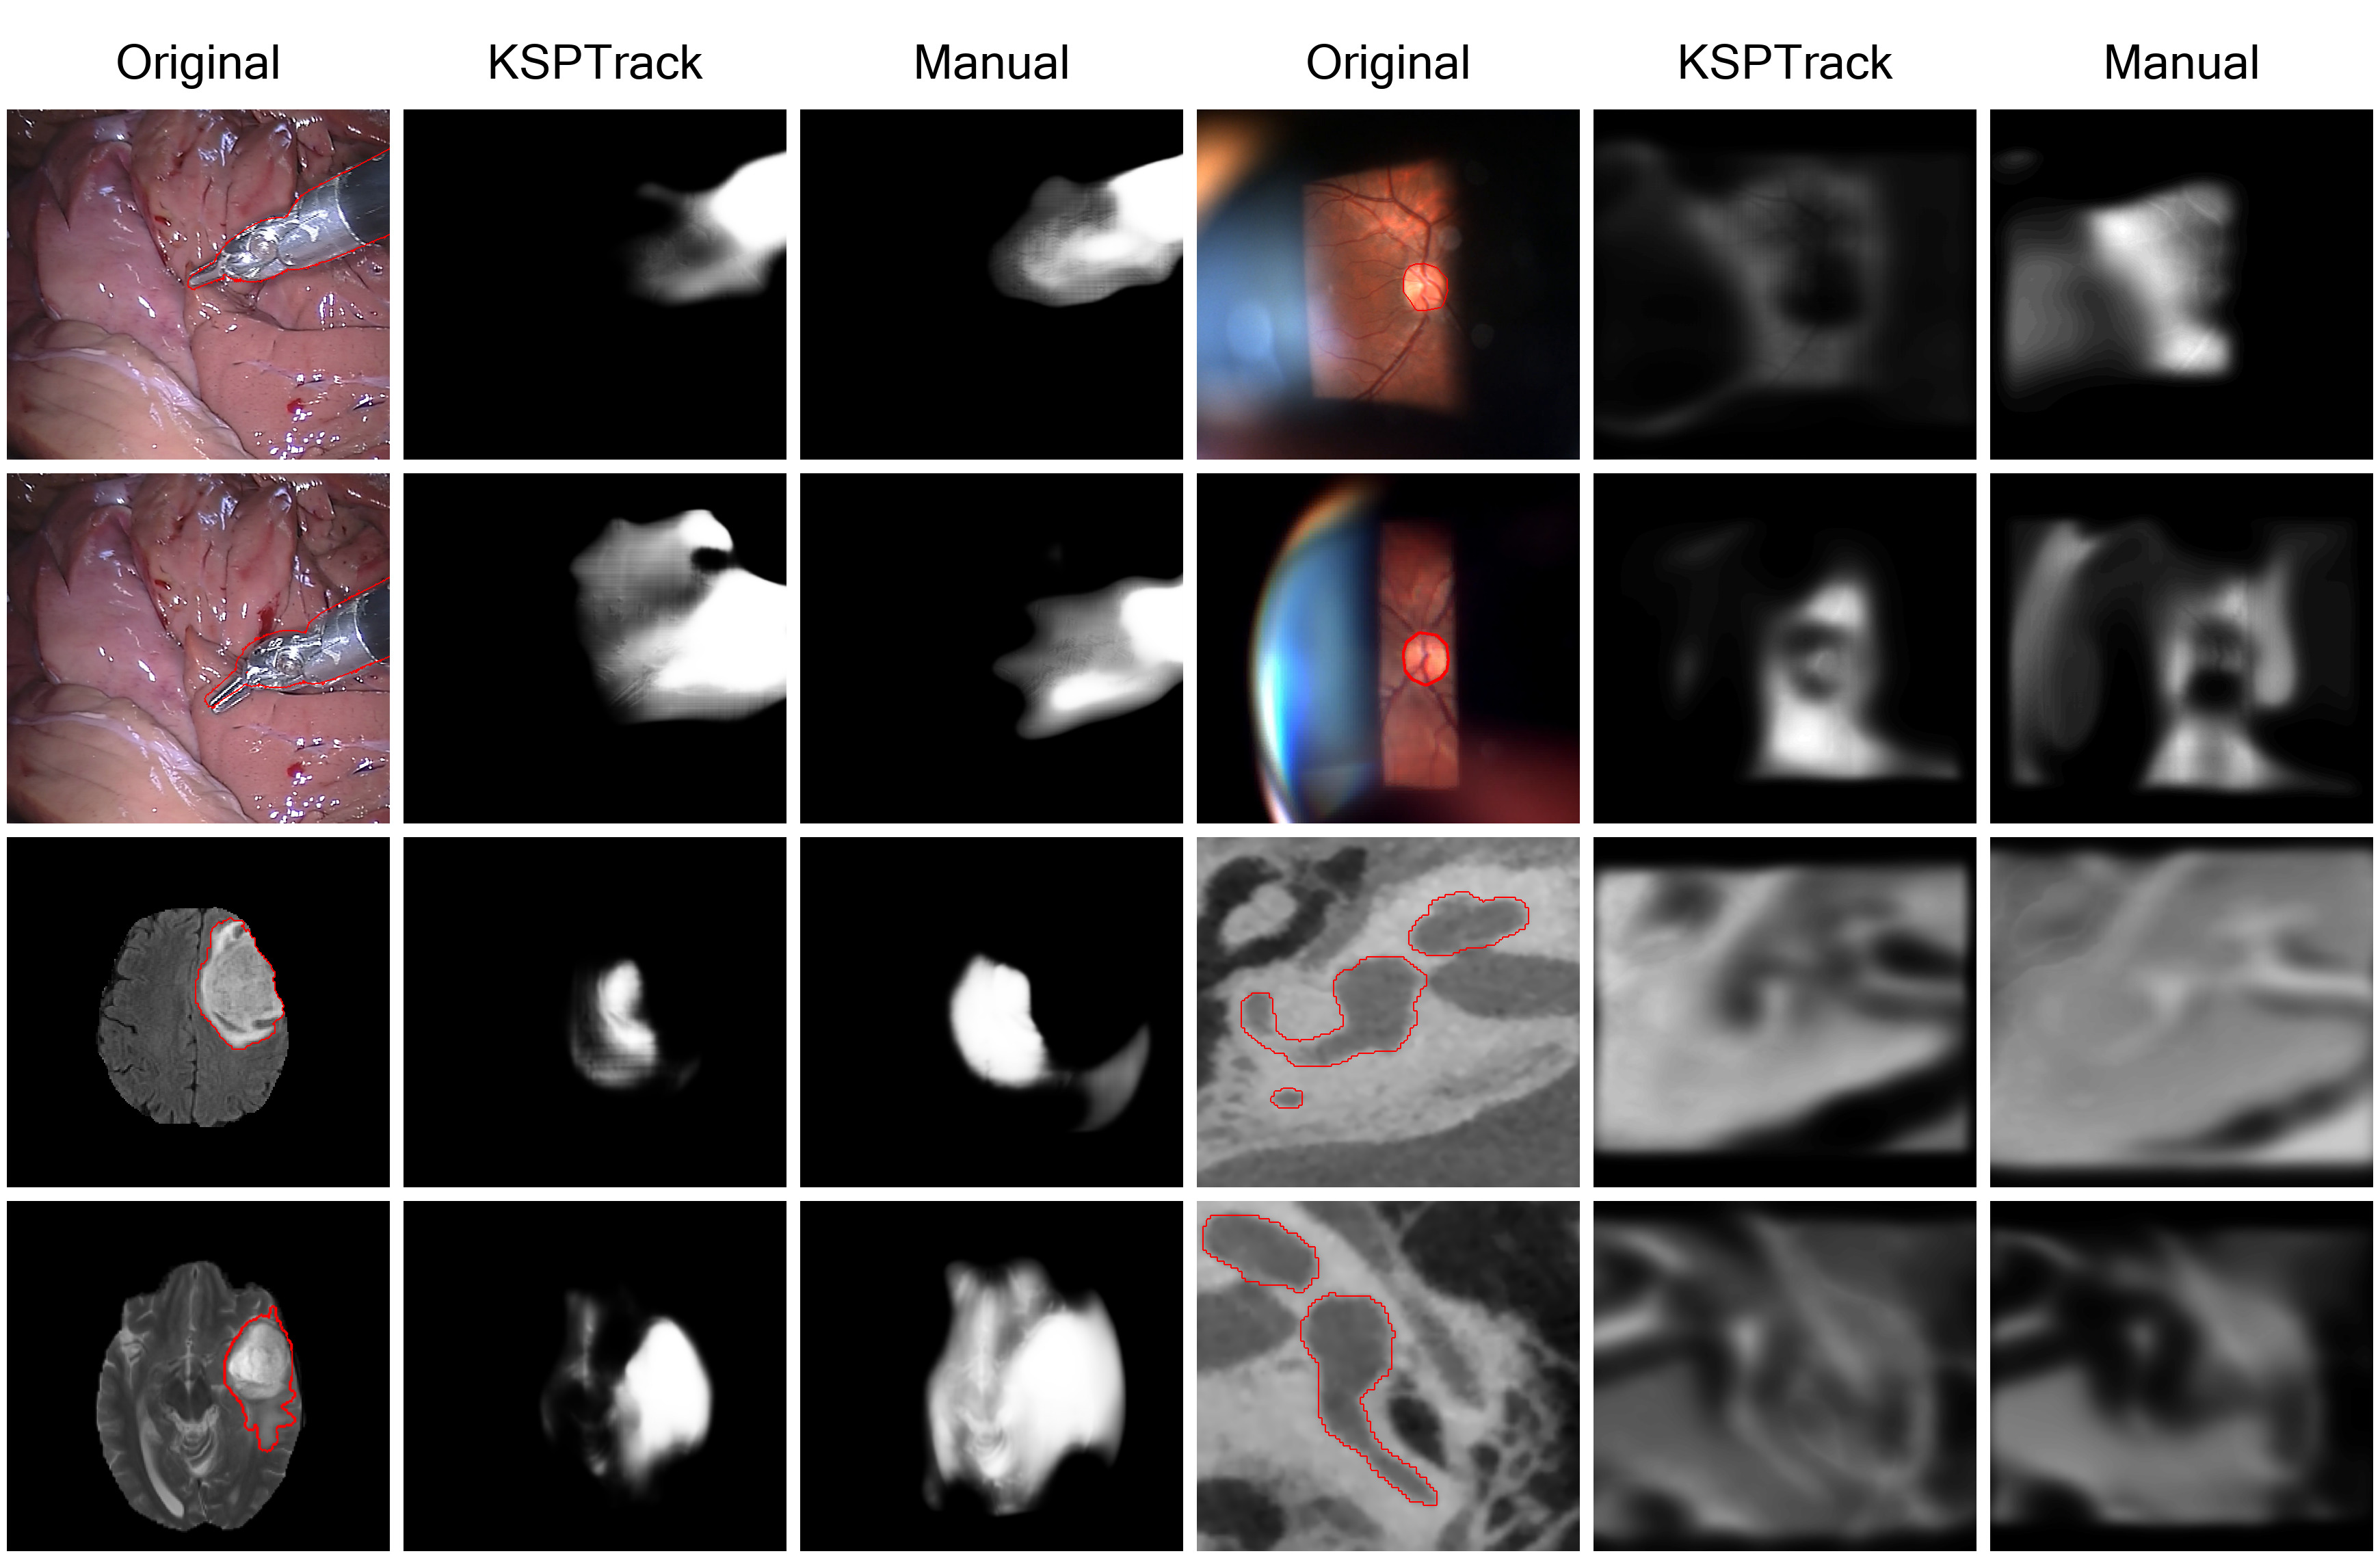
\includegraphics[width=0.99\textwidth]{fig10}
\caption{Maximum F1 scores when using \KSPnb or manual segmentations to train a supervised CNN for pixel wise predictions.}
\label{fig:learning}
\end{figure}

\subsection{Experiment 3: Impact of coverage ratio and supervision}
When dealing with relatively large objects, it is quite possible that only the most salient parts of the object would be provided as locations, leaving large or homogeneous parts of the object unobserved. This is predominant in the case of the {\bf Tweezer} image sequence where a larger part of the shaft is often distant from any given $g_t$. In this experiment, we are interested in knowing to what degree the supervised 2D locations play a role in the quality of the segmented objects.

To estimate the impact of this effect, we evaluate the segmentation performance of our method as function of the coverage ratio (\ie ratio of the covered area over the total area of the object).
In this setting, we first selected a reference frame where the object appears in its entirety. We then manually select a set of positive superpixels from other frames so as to cover a pre-defined coverage ratio of the object surface. Note that only a single 2D location is still provided on each frame but that it is the entire set that specifies the coverage proportion of the object.
Each one of the $4$ sequences of the {{\bf Tweezer} dataset were assigned $5$ sets of 2D locations, each corresponding to approximately $\{20, 40, 60, 75, 90\}\%$ of the total area of the object (see Fig.~\ref{fig:coverage}, Left).

We report the F1 score with respect to the coverage ratio in Fig.~\ref{fig:coverage}(Right). As our method does not resort to frame-wise filling, we observe that the coverage ratio affects the F1-score as only ``seen'' regions end up being segmented. As such, attempting to recover the entire object over all frames from a few points remains extremely difficult. We note that even at $90\%$ coverage ratio, the F1 score is of roughly $0.82$ and not higher. As can be observed in the bottom right frame of Fig.~\ref{fig:coverage}(Left), this is largely due to oversegmentations introduced by the superpixels used.
\begin{figure}
\centering
\begin{subfigure}{.49\textwidth}
  \centering
  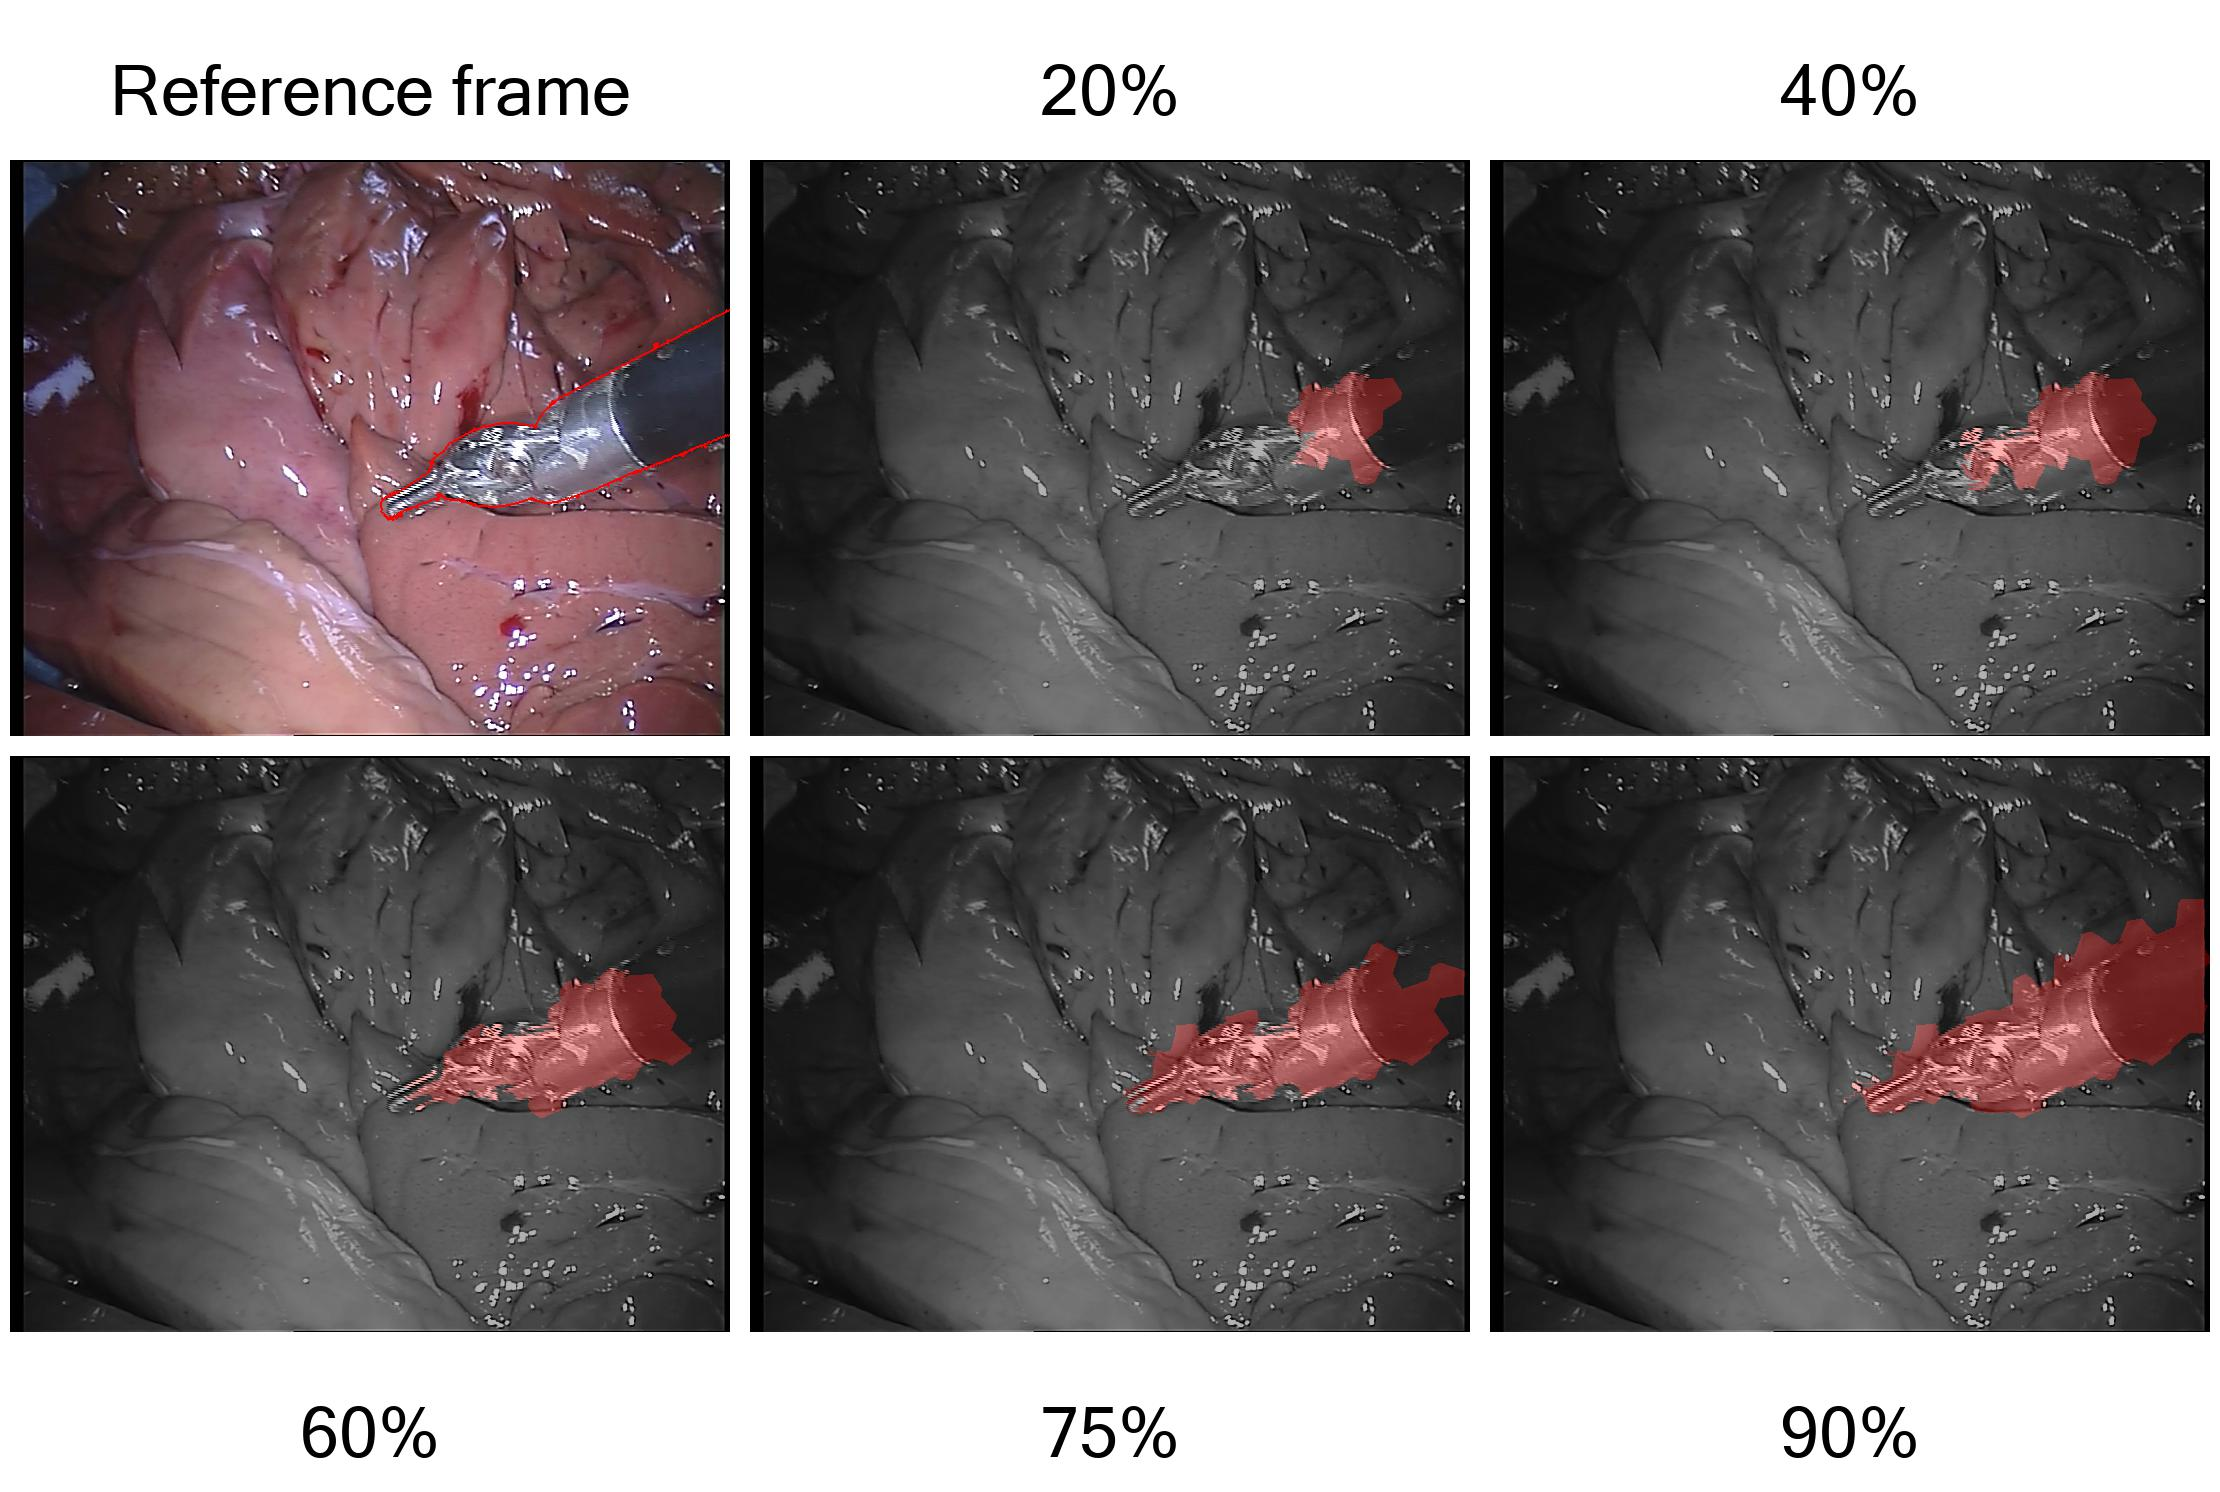
\includegraphics[width=\linewidth]{fig11a}
  \label{fig:sub2}
\end{subfigure}
\begin{subfigure}{.49\textwidth}
  \centering
  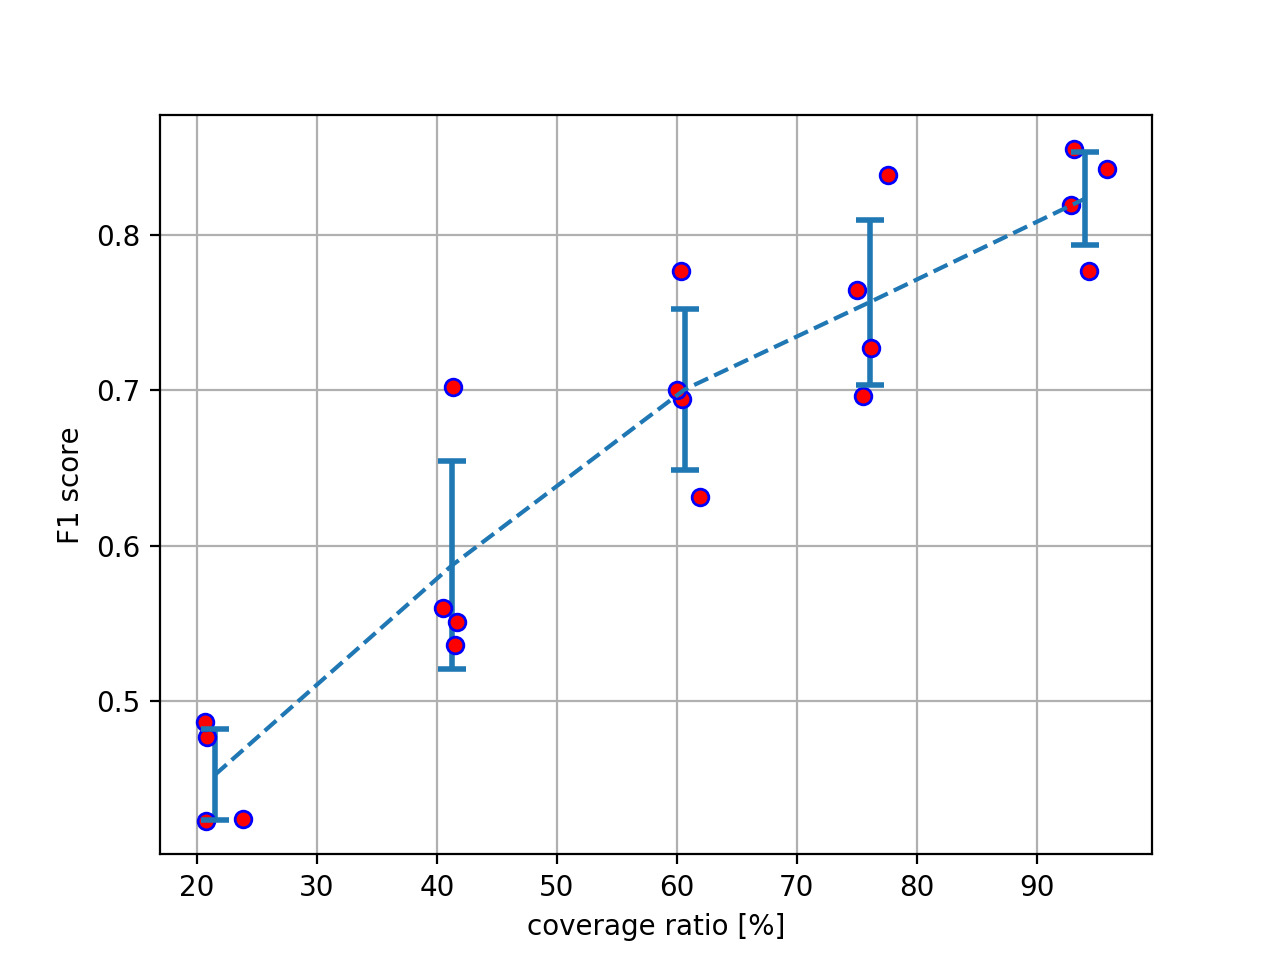
\includegraphics[width=\linewidth]{fig11b}
  \label{fig:sub1}
\end{subfigure}%
\caption{(Left) Graphical examples of coverage ratio for a Tweezer sequence using each of the following ratios: $20$, $40$, $60$, $75$, and $90\%$. (Right) Boxplot of F1 scores with respect to coverage ratio on a Tweezer sequence. 
}
\label{fig:coverage}
\end{figure}

\begin{figure}[t]
\centering
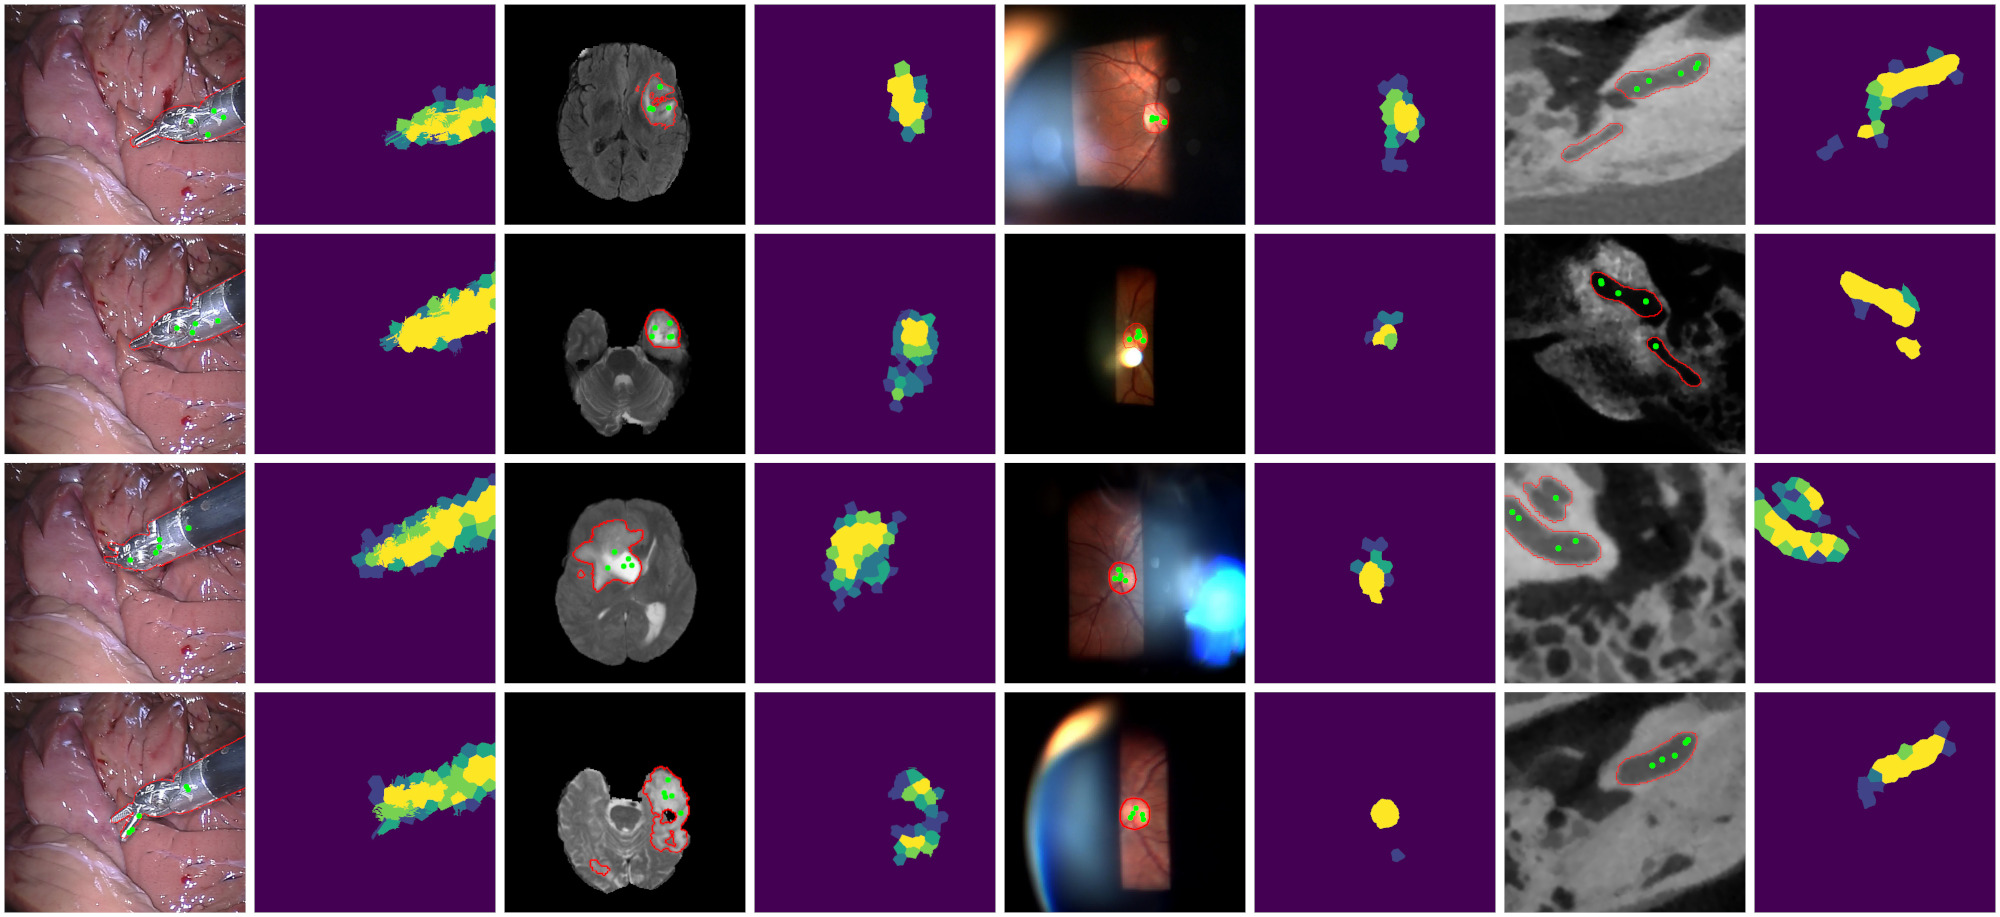
\includegraphics[width=0.97\textwidth]{fig12}
\caption{Qualitative results of our approach when using different sets of supervised 2D locations. Columns 1, 3, 5, and 7 show the original image with highlighted ground truth contour in red. The 2D locations are in green. Columns 2, 4, 6, and 8 show the mean of all binary segmentations over $5$ sets of 2D locations.}
\label{fig:multigaze}
\end{figure}

In addition, Fig.~\ref{fig:multigaze} shows the mean segmentation over 5 different sets of provided 2D locations. We observe the largest inter-set variability on the {\bf Cochlea} dataset, where a standard deviation ranging from $5\%$ to $16\%$ is observed. The lowest variability is attained on the {\bf Tweezer} dataset within $2\%$ to $4\%$ range. The latter results can be explained by the fact that the {\bf Cochlea} dataset gives different possibilities as to which branch of the cochlea will be observed. In contrast, the {\bf Tweezer} dataset shows a stable appearance and shape throughout the sequences, thereby limiting the inter-user variability as each set covers roughly the same regions of the object.

\subsection{Experiment 4: Image-Object Features}
We also wish to assess the gain in performance of the proposed IOS method with respect to simpler approaches. In particular, we compare produced segmentation performances when using the following alternatives:
\begin{itemize}
\item[-]{\bf{U-Net:}} Using the same architecture as presented in Sec.~\ref{sec:features} in combination of a simple $L^2$ reconstruction loss,
    \begin{equation}
    \mathcal{L}' = \sum_{{I}_t \in \mathcal{I}} \sum_{k,l} \| I_t(k,l) - {\hat{I}}_t(k,l)\|^2.
    \label{eq:loss_features}
    \end{equation}
    \noindent
    This is similar to our object-image features, but without the object prior given by the 2D locations.
  \item[-]{\bf{OverFeat:}} We use the pre-trained CNN of~\cite{sermanet13}. The model is trained in a supervised classification setup on the ImageNet 2012 training set \cite{deng09}, which contains about $1.2$ million natural images from $1000$ classes. In our setup, we use the provided \textit{fast} model, and extract square patches centered on the centroids $r_t^n$. We set the size of patches so as to include all pixels in superpixel $s_t^n$. The patch is then resized to ($231 \times 231$) and fed into the network to give a feature vector of size $4096$ at the output of the penultimate layer.
\end{itemize}

Table~\ref{tab:multigaze} shows the maximum F1-score and standard deviation when using different features in \KSP . Here we show the performance of each feature type over each sequence for each dataset. On average, IOS features provides superior performances over alternatives. In some cases (\eg Brain dataset), the standard U-Net or Overfeat features appear to perform better on two sequences in particular. Naturally, the performance variance with IOS features is higher given that they depend on the provided 2D locations. 

\begin{table}
\centering
\losscomp
\caption{Quantitative results of \KSPnb with different feature used on all datasets with five sets of 2D locations per sequence. Mean and standard deviationm F1 scores are given for 2D locations sets.}\label{tab:multigaze}
\end{table}

\subsection{Experiment 5: Impact of outliers and missing 2D locations}

Next, we look at the effect of the quality and quantity of provided 2D locations, that may vary in practice depending on various factors (\eg speed of object, gaze-tracker calibration accuracy etc.). To do this, we produce noisy versions of the 2D locations used in Sec.~\ref{sec:accuracy}. In particular, we generate for a given outlier proportion $\delta \in \{5, 10, 20, 40, 50 \} \%$, three sets of 2D locations. The first samples outliers uniformly on the background, the second samples uniformly on a neighborhood of the object at a distance of $5\%$ (normalized w.r.t. largest dimension of the image), and the last samples at a distance of $10\%$.
Examples for the last two cases are illustrated in Fig.~\ref{fig:neigh_5} and~\ref{fig:neigh_10}, respectively.
We also show the case where a proportion of 2D locations are missing entirely.
Fig.~\ref{fig:outliers} depicts the F1 score with respect to the proportion of outlier or missing locations on the {\bf Tweezer} sequence \#1.
We report for missing 2D locations a maximum decrease in F1 score of $12\%$ when $40\%$ of locations are missing. This showcases the robustness of our method brought by the global data association optimization. Outliers however impact our method more severely as for incorrect 2D locations of up to $ 5\%$ decrease performances by $14\%$ with $20\%$ of incorrect locations. Similarly, with errors at a maximum of the $10\%$ distance, the performance decreases by $18\%$ when $40\%$ of the locations are corrupted. For severe corruptions of $50\%$ over the entire background, then the performance drops by $45\%$. 
In general however, we note that the performance remains acceptable up to a $40\%$ outlier proportion. This is explained by the fact that our foreground model effectively penalizes such outliers through its bagging component.

\begin{figure}
\centering
\begin{subfigure}[t]{.25\textwidth}
  \centering
  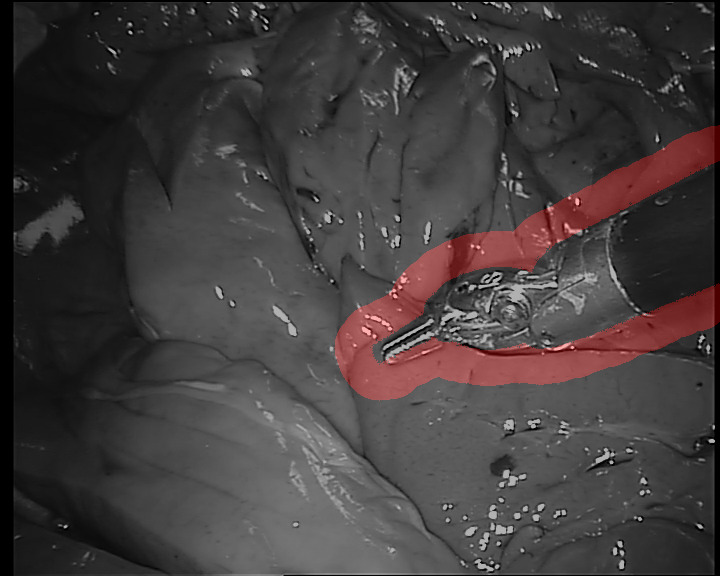
\includegraphics[width=\linewidth]{fig13a}
  \caption{\label{fig:neigh_5}}
\end{subfigure}
\begin{subfigure}[t]{.25\textwidth}
  \centering
  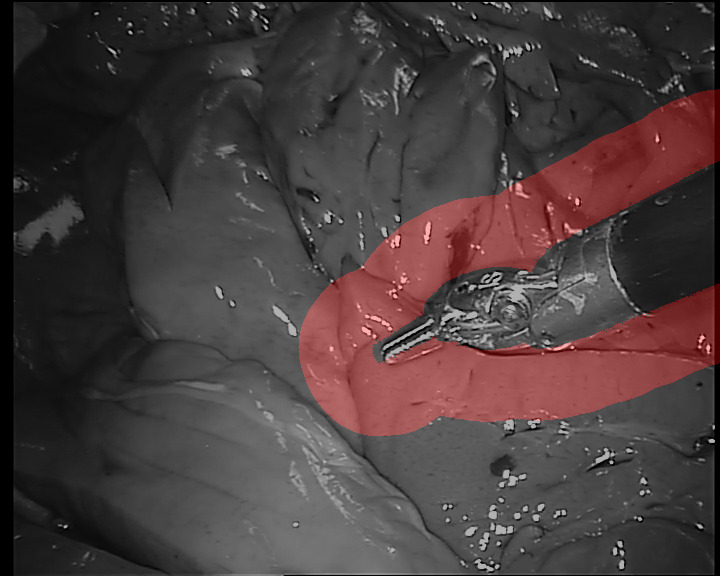
\includegraphics[width=\linewidth]{fig13b}
  \caption{\label{fig:neigh_10}}
\end{subfigure}%
\begin{subfigure}[t]{.4\textwidth}
  \centering
  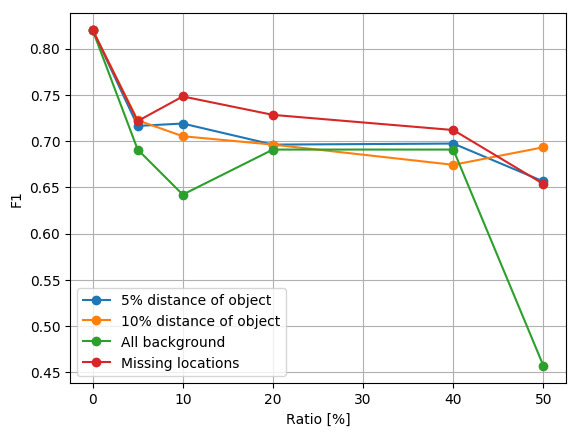
\includegraphics[width=\linewidth]{fig13c}
  \caption{\label{fig:outliers}}
\end{subfigure}%
\caption{
(a and b) Example frames with outlier regions highlighted in red corresponding to distance of $5\%$ and $10\%$, respectively. (c) F1 scores with respect to the corrupted proportion of provided 2D locations.\label{fig:outliers_missing}
}
\end{figure}
%%% Local Variables:
%%% mode: latex
%%% TeX-master: "../../main"
%%% End:
